% !TEX root =./main.tex
\section{Block 2 : Time Gain Compensation}

    \subsection{Theory}
    As sound travels, it attenuates through geometric spreading.  As a result, the magnitude of the second reflected pulse is significantly lower. Therefore, the program must compensate to increase the magnitudes of the two pulses back to the original magnitude of 1. 
    The samples must first be converted into distance. This is easily accomplished using the following conversion.
    \begin{align*}
     \frac{\text{Sample Index}}{F_s} \cdot c_{\text{sound}}    
    \end{align*}
    

    For omni directional transducers the inverse-square law $(I \propto  \frac{1} {r^2} )$ dictates how the signal degregatates with time. However, this signal was relativley directional and only degragated by $r$. I order to reduce the effects, the samples were multiplied by $r$. Thus using a linear function to increase the magnitude of the first and second pulses.  


    \subsection{Analysis}

    \begin{figure}[H]
        \centering
        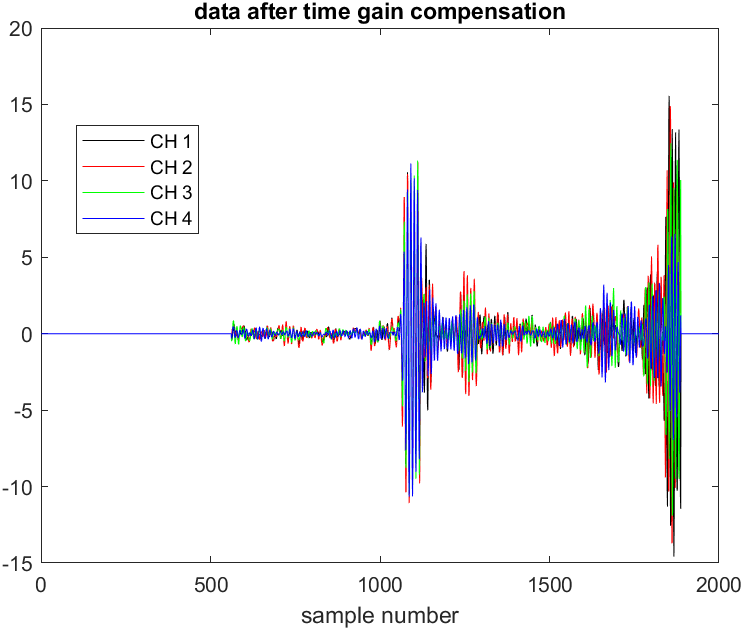
\includegraphics[width=0.5\linewidth]{figures/time_gain_1.png}
        \caption{Data after time gain compensation}
        \label{fig:time_gain1}
    \end{figure}

    \ref{fig:time_gain1}

